\chapter{Meilensteinberichte}
\label{app:meilensteinberichte}
In diesem Kapitel werden die einzelnen Berichte der Meilensteine aufgeführt. Diese sollen Aufschluss über den Stand des
Projektes während der Umsetzung geben.

\section{Meilensteinbericht M1 vom 26. September 2019}
In der Phase bis zum ersten Meilenstein ging es darum das Projekt zu starten sowie die Initialisierungsphase
einzuläuten. Ziel dieses ersten Eckpunktes war, sich nochmals genau mit der Aufgabenstellung zu befassen und allenfalls
Unklarheiten mit dem Projektbetreuer zu klären. Ausserdem sollte zum Ende dieser Phase die Aufgaben der
Initialisierungsphase aufgeteilt sein.

\subsection{Aktueller Stand bei Meilenstein}
Alle vorgenommenen Aufgaben, welche in diesem Meilenstein zu erledigen waren, konnten abgeschlossen werden. Die
Aufgabenstellung war klar und es war deutlich was in der Initialisierungsphase des Projektes zu tun war.

\subsection{Ausblick zum nächsten Meilenstein}
Da alle Aufgaben des aktuellen Meilensteins erledigt werden konnten, müssen keine Aufgaben in den nächsten Meilenstein
übernommen werden.

\section{Meilensteinbericht M2 vom 10. Oktoper 2019}
In der Phase bis zum Meilenstein M2 soll die Initialisierungsphase abgeschlossen werden. Diese beinhaltet, dass die
Fragestellung des Projektes nochmals genau durchgearbeitet wird, allfällige Fragen geklärt werden und vor allem
Eckpunkte des Projektes definiert werden.

\subsection{Aktueller Stand bei Meilenstein}
In diesem Meilenstein konnte alle Aufgaben der Initialisierungsphase abgeschlossen werden, die Aufgabenstellung wurde
nochmals gründlich untersucht und verschiedene Fragen die währenddessen aufgetaucht sind, geklärt. Ausserdem wurde sich
darauf geeinigt, dass die Sprache des Projektes Deutsch ist und auch der Prototyp für die Deutsche Sprache entwickelt
werden soll.

\subsection{Ausblick zum nächsten Meilenstein}
Da in dieser Phase alle Aufgaben erledigt werden konnten, müssen keine Tasks in die nächste Phase übernommen werden und
der Meilenstein kann abgeschlossen werden. Ausserdem wird mit dem Abschluss dieses Meilensteins die Ideenfindungsphase
gestartet.

\section{Meilensteinbericht M3 vom 21. Oktober 2019}
In der Phase bis zum Meilenstein M3 soll die divergierende Ideenfindungsphase abgeschlossen werden. Diese Phase
beinhaltet, dass der aktuelle Stand der Technik untersucht wird und verschiedene aktuelle Ansätze erforscht werden.
Diese Phase soll auch dazu dienen, erste Experimente bezüglich der Aufgabenstellung durchzuführen um die Machbarkeit der
verschiedenen Ansätze zu beurteilen.

\subsection{Aktueller Stand bei Meilenstein}
In diesem Meilenstein wurden viele verschiedene Ansätze für die Umsetzung des Projektes untersucht und auch einige
wenige Experimente durchgeführt. Während dieser Phase wurde sehr schnell klar, dass es viele verschiedene Möglichkeiten
gibt die Problemstellung zu lösen. Daher wurde entschieden, dass der Fokus der Ideenfindung auf dem Bereich des Neuronal
Style Transfer liegt und sich die Ideenfindung eher auf die Untersuchung verschiedener Style Transfer Modelle
beschränken sollte. Dadurch konnten in der Ideenfindungsphase, viele verschiedene Modelle anhand deren
wissenschaftlichen Arbeiten beurteilt werden.

\subsection{Ausblick zum nächsten Meilenstein}
Der Meilenstein wurde erreicht, durch das erfolgreiche Finden verschiedener Ansätze die eine vielversprechende Lösung
für das Projekt bieten. In der nächsten Phase wird es deutlich ob die verschiedenen Modelle Erfolgschancen bieten.

\section{Meilensteinbericht M4 vom 11. November 2019}
In der Phase bis zum Meilenstein M4 soll die konvergierende Ideenfindungsphase abgeschlossen werden. Diese Phase
beinhaltet, dass die gefundenen Modelle aus der divergierenden Ideenfindungsphase, bezüglich der Umsetzbarkeit und
Anwendbarkeit auf das Projekt, beurteilt werden sollen. Ausserdem sollte ein Datenkorpus gewählt werden für das Projekt,
um die jeweiligen Modelle damit zu trainieren.

\subsection{Aktueller Stand bei Meilenstein}
In diesem Meilenstein konnten die in der vorherigen Phase gefundenen Modelle beurteilt werden. Dabei wurde vor allem
bemerkt, dass die Auswahl des Datenkorpus eine der wichtigsten Entscheidungen ist, die in unserem Projekt getroffen
werden muss. Denn durch die gewählten Daten wird auch entschieden welche Modelle überhaupt in Frage kommen, z.B. ist
eine der Entscheidung welche getroffen werden muss ob es sich bei um parallele Daten oder nicht handelt. Die Sprache des
Korpus wurde bereits in einer vorherigen Phase definiert und somit wurde die Auswahl auch eingeschränkt. Geeinigt wurde
sich auf einen deutschen nicht parallelen Korpus bestehend aus Sätzen eines Kinderlexikons und Wikipedia, um einen
genügend grossen Unterschied zu erhalten. Anschliessend konnten auch verschiedene Modelle ausgeschlossen werden, welche
einen parallelen Datenkorpus benötigen. Bis zum Schluss hatten wir noch 2 Modelle (ControlGen und CrossAlign), welche
unseren Anforderungen entsprachen und auch mit den Daten von uns arbeiten können.

\subsection{Ausblick zum nächsten Meilenstein}
Der Meilenstein M4 konnte erreicht werden, vor allem durch die Entscheidung sich zuerst auf die Auswahl der Daten zu
konzentrieren und erst anschliessend auf die Auswahl der Modelle. In dieser Phase konnten sehr viele wichtige
Erkenntnisse über das Trainieren der Modelle und der breite der Modelle gewonnen werden.

\section{Meilensteinbericht M5 vom 9. Dezember 2019}
Bis zum Meilenstein M5 soll die Umsetzungsphase abgeschlossen sein, es soll also ein funktionsfähiger Prototyp zur
Verfügung stehen, welcher die Problemstellung ansatzweise löst. Dieser Prototyp soll mit den erforschten Modellen
entwickelt werden und die gelernten Erkenntnisse aus vorherigen Phasen angewandt werden. Ausserdem soll die
Dokumentation der ganzen Arbeit in einer ersten Fassung vorliegen, so dass mit dem Gegenlesen und Korrigieren angefangen
werden kann.

\subsection{Aktueller Stand bei Meilenstein}
Die Aufgaben in diesem Meilenstein konnten nicht vollständig erreicht werden, da sehr viel Zeit verloren ging beim
Testen der beiden Modelle, um die optimalen Hyperparameter zu finden. Der Grund dafür war, dass das nötige Wissen über
das Trainieren von \gls{GAN} fehlt und dadurch die Graphen der einzelnen Modelle schlecht interpretiert werden konnten. Daher
wurde im Gespräch mit dem Projektbetreuer versucht von diesem Wissen zu profitieren, so dass die nächsten Modelle besser
interpretiert werden können. Durch das viele probieren der Hyperparameter konnten noch keine Fortschritte bei der
Entwicklung des Prototypen gemacht werden.

\subsection{Ausblick zum nächsten Meilenstein}
Der Meilenstein konnte nicht erreicht werden, da Artefakte wie der Prototyp oder das vollständige Testen der Modelle
nicht vorliegen. Dadurch müssen diese Aufgaben in den nächsten Meilenstein einfliessen und erledigt werden. Obwohl der
Meilenstein nicht erreicht wurde, ist unser Wissen über \gls{GAN} und ihr Training extrem gestiegen, so dass wir
zuversichtlich sind diese in der nächsten Phase zu meistern. Die Dokumentation wurde durch diese Probleme auch ein wenig
zurückgestellt und muss in dem letzten Meilenstein nochmals aufgenommen werden.

\section{Meilensteinbericht M6 vom 20. Dezember 2019}
Der Meilenstein M6 ist der letzte im Projekt und bis dorthin muss die Dokumentation fertig sein, sowie ein
funktionsfähiger Prototyp vorliegen. In dieser Phase geht es vor allem um die Finalisierung des Dokumentes und
Prototypes.

\subsection{Aktueller Stand bei Meilenstein}
Im letzten Meilenstein mussten die Artefakte, welche in der vorherigen Phase nicht zu Stande kamen, als erstes
erarbeitet werden. Zunächst konnten nochmals verschiedene Versionen der Modelle erstellt, interpretiert und verglichen
werden. Dies konnte nur mithilfe der vorher gewonnen Erkenntnisse geschehen. Danach konnte relativ schnell der Prototyp
geschrieben werden, weil dieser auf das Minimum an Funktionalität reduziert wurde. Und zum Schluss wurde noch die
Dokumentation über das Projekt fertiggestellt und der Meilenstein somit erreicht werden.

\chapter{Recherche}
\label{app:recherche}

\section{Links}
\begin{itemize}
    \item List of various useful links: <https://github.com/fuzhenxin/Style-Transfer-in-Text>
\end{itemize}

\section{Arbeiten}
All paper listed. Every paper will assigned a number to make communication easier. Papers are tried to be hold in
categories.

\subsection{Overview - Neural Style Transfer}
Papers which describe neural style transfer in general and show a general overview over the existing technologies and
ideas.

\subsubsection{01 - What is wrong with style transfer for texts?}
\textbf{Link: } <https://arxiv.org/pdf/1808.04365.pdf>
\newline
\newline
Das Paper bietet eine gute Übersicht über die aktuelle Lage mit dem Thema Neural Style Transfer. Die Übersicht wird
unter der Frage nach den schwächen des Bereichs.
\newline
\newline
Dabei wird eine Übersicht über die vorhanden vorgeschlagenen Modelle gegeben.
\begin{itemize}
    \item \textbf{Ad-hoc defined:} Der Style Transfer erfolgt über ein Datenset eines Autoren oder Platform. Dabei wird
    versucht der Stil des Datenset wiederzugeben. Dabei wird, z.B. mit einem LSTM, ein neuer Text aus dem Set generiert.
    Es handelt sich somit um die generierung von neuem Text aufgrund eines Datensatz.
    \item \textbf{Neural Machine Translation (NMT):} Die Stile werden als Sprachen angesehen. Dabei wird ein Übersetzer
    für den einen in den anderen Stil (Sprache) verwendet. So mit kann mithilfe eines parallen Datensatzes stilisiert
    werden.
    \item \textbf{Post NMT:} Allgemein wurde sich geeinigt das der Style Transfer nicht aufgrund von Fragementen
    getätigt werden soll. Eher soll der Transfer aufgrund der Daten parametrisiert werden. Dieser Ansatz wird momentan
    stark weiterverfolgt und erweitert.
\end{itemize}
Weiter wird im Paper die Problemstellung der Definition für Text-Semantik und Text-Stil aufgeführt.

\subsubsection{03 - A Neural Algorithm of Artistic Style}
\textbf{Link: } <https://arxiv.org/abs/1508.06576>
\newline
\newline
Das Paper bietet die Grundlagen für Neural Style Transfer. Dabei wird die Technik anhand von Transfer von artistischem
Stil anhand von Gemälden und Bilder eingeführt.
\newline
\newline
Das Paper ist relevant da oft zitiert und als eigentlicher Ursprung der Technik gehandelt.

\subsection{Domain Adaptive Approach}

\subsubsection{02 - Domain Adaptive Style Transfer}
\textbf{Link: } <https://arxiv.org/abs/1908.09395>
\newline
\newline
Dieses Modell versucht aufgrund von eines nicht parallelen domain-übergreifenden Datensets den Stil daraus zu
parametrisieren.
\newline
\newline
Der Ansatz ist interessant, da der zu Datensatz geringe Mengen an Domain spezifischen Daten benötigt.

\subsection{Latent Representation Approach}

\subsubsection{04 - Controllable Unsupervised Text Attribute Transfer via Editing Entangled Latent Representation}
\textbf{Link: } <https://arxiv.org/abs/1905.12926>
\newline
\newline
In diesem Ansatz wird versucht der Latent Space (Feature Space) mit Gewichtung zu kontrollieren. Dadurch kann ein Input
auf verschiedene weisen interpretiert werden. Dabei repräsentiert das Gewicht, wie stark der Text vom Source-Style zum
Target-Style stilisiert werden soll.
\newline
\newline
Der Ansatz ist interessant, da eine Abstufung des Stils möglich ist. So könnte eventuell die Bewertung beibehalten
werden.

\subsubsection{05 - Evaluating prose style transfer with the Bible}
\textbf{Link: } <https://arxiv.org/abs/1711.04731>
\newline
\newline
In dieser Forschungsarbeit geht es darum, dass ein System, welches mit einem Input Text und einem Zielprosa-Stil
versorgt wird, eine Ausgabe liefert, die die Bedeutung des Eingabetextes bewahrt, aber den Stil ändert. Um das Modell zu
trainieren wird ein paralleler Datenkorpus benötigt, in diesem Beispiel wird die Bibel in verschiedenen Ausführungen als
qualitativ hochwertiger Korpus genutzt. Als Metriken werden \gls{BLEU} und PINC verwendet.
\newline
\newline
Da der Datenkorpus qualitativ sehr hochwertig ist, kann dieser Korpus auch für weitere Modelle verwendet werden. Jedoch
wird in unserer Arbeit ein deutscher Datenkorpus angestrebt. Dennoch ist die Idee die Bibel als parallele Datensammlung
zu verwenden interessant und wird mit deutschen Editionen weiter untersucht.
\newline
\newline
Ausserdem werden in dieser Schriftstück wertvolle Referenzen auf andere Arbeiten genannt, welche sich mit einigen Themen
des Style Transfers noch tiefer auseinander gesetzt haben. Diese Referenzen sollten weiter untersucht werden.
\newline
\newline
Das grösste Problem von Style Transfer wird hier immer wieder angesprochen, nämlich die mangelhafte Anzahl parallellen
Datenkorpusse.

\section{Metriken}

\subsection{BLEU Score}
\textbf{Links:}
\begin{itemize}
    \item https://towardsdatascience.com/evaluating-text-output-in-nlp-bleu-at-your-own-risk-e8609665a213
    \item https://www.sdl.com/blog/understanding-mt-quality-bleu-scores.html
\end{itemize}

\chapter{Arbeitsjournal}
\label{ch:arbeitsjournal}
In diesem Kapitel wird das Arbeitsjournal, welches im Rahmen des Projektes geführt wurde, dargestellt. Es soll aufzeigen
wie die Arbeit des Projektes auf die zwei Studenten verteilt wurde. Das Projekt wurde in mehrere grössere Teile
zusammengefasst und im Journal aufgelistet, so dass das Arbeitsjournal möglichst kompakt und simpel gehalten werden
konnte. Die Auflistung wurde an den Aufbau des Projektes und die vier Git Repositories angelegt. Um detailliertere
Angaben zur Aufgabenverteilung und deren Umsetzung zu erhalten können in den Git Projekten die Commits verfolgt werden
unter:
\begin{enumerate}
    \setlength\itemsep{0em}
    \item \hyperlink{https://gitlab.enterpriselab.ch/Pwn3rs/wipro-doc}{wipro-doc}
    \item \hyperlink{https://gitlab.enterpriselab.ch/Pwn3rs/wipro-data}{wipro-data}
    \item \hyperlink{https://gitlab.enterpriselab.ch/Pwn3rs/wipro-source}{wipro-source}
    \item \hyperlink{https://gitlab.enterpriselab.ch/Pwn3rs/wipro-logs}{wipro-logs}
\end{enumerate}
\noindent
In der Tabelle \ref{tab:arbeitsjournal} ist das Arbeitsjournal des Projektes aufgelistet, wobei in der Spalte
\textit{Student} das Kürzel des jeweiligen Studenten verwendet wurde. RB für Reto Barmettler und FG für Fabian Gröger.

\begin{table}[ht]
    \centering
    \begin{adjustbox}{angle=90}
        \begin{tabular}{|l|l|l|c|c|}
        \hline
        \textbf{Arbeit} & \textbf{Details} & \textbf{Projekt} & \textbf{Student} & \textbf{Stunden} \\
        \hline
        Git Repositories & Pflegen der Git Repositories & gitlab & RB, FG & 10h \\
        \hline
        Dokumentation & Dokumentieren der Arbeit & wipro-doc & RB, FG & 110h \\
        \hline
        Projektmanagement & Managen des ganzen Projektes & wipro-doc & RB & 5h \\
        \hline
        Recherche & Recherche zur Problemstellung & wipro-doc & RB, FG & 10h \\
        \hline
        Recherche & Recherche zum Neural Style Transfer & wipro-doc & RB, FG & 20h \\
        \hline
        Recherche & Recherche zu Modellen von \gls{NST} & wipro-doc & RB, FG & 30h \\
        \hline
        Datensatz & Idee welchen Datensatz verwenden & wipro-data & RB, FG & 10h \\
        \hline
        Datensatz & Daten von Internet crawlen & wipro-data & FG & 5h \\
        \hline
        Datensatz & Daten aufbereiten, säubern & wipro-data & RB & 15h \\
        \hline
        Datensatz & Daten statistisch analysieren & wipro-data & RB & 10h \\
        \hline
        Datensatz & Daten aufbreiten für Weiterverarbeitung & wipro-data & RB & 5h \\
        \hline
        Modelle & Bestehendes GitHub Projekt integriert & wipro-source & RB, FG & 5h \\
        \hline
        Modelle & Anpassungen an den Modellen & wipro-source & FG & 15h \\
        \hline
        Modelle & Training der Modelle & wipro-source & FG & 15h \\
        \hline
        Prototyp & Erstellen des Prototypen & wipro-source & RB, FG & 10h \\
        \hline
        Evaluation & Bewerten der Resultate der Modelle & wipro-logs & RB, FG & 20h \\
        \hline
        Evaluation & Evaluieren der Resultate der Modelle & wipro-logs & RB, FG & 20h \\
        \hline
        Docker & Dockerfile für Prototypen & wipro-source & FG & 5h \\
        \hline
        \end{tabular}
    \end{adjustbox}
	\caption{Arbeitsjournal}
	\label{tab:arbeitsjournal}
\end{table}

\chapter{Anleitung Installation Prototyp}
\label{ch:anleitung_proto}
In diesem Abschnitt wird die Installation des Prototypen genau beschrieben. Der Installationsprozess gestaltet sich
relativ simpel, weil dieser in ein Docker Image gepackt wurde.
\newline
\begin{enumerate}
    \item Als erstes muss gewährleistet werden, dass Docker korrekt installiert ist und eine konstante
    Internetverbindung besteht. Wenn diese beiden Punkte sichergestellt wurden, kann mit dem zweiten Schritt
    weitergemacht werden.
    \item Danach muss nur noch der Docker Container von Docker Hub gepullt werden, dies geschieht mittels diesem Command:
    \begin{verbatim}
    docker run \
    -it --name wipro-prototype \
    -e LANG=C.UTF-8 \
    fabiangroeger96/wipro-prototype:1.0.2
    \end{verbatim}
    Dieser holt sich die Version $1.0.2$ von Docker Hub und führt diese gleich aus, mit einer interaktiven Shell
    gekoppelt.
    \item Nach dem Starten des Docker Containers wird sogleich der Prototyp gestartet und dieser kann verwendet werden.
    \item Um den Prototypen zu beenden, kann das Keyword \verb|exit| verwendet werden
    \item Nach dem Benutzen des Docker Images kann dieses mittels dem folgenden Befehl gelöscht werden
    \begin{verbatim}
    docker rm -f wipro-prototype
    \end{verbatim}
\end{enumerate}


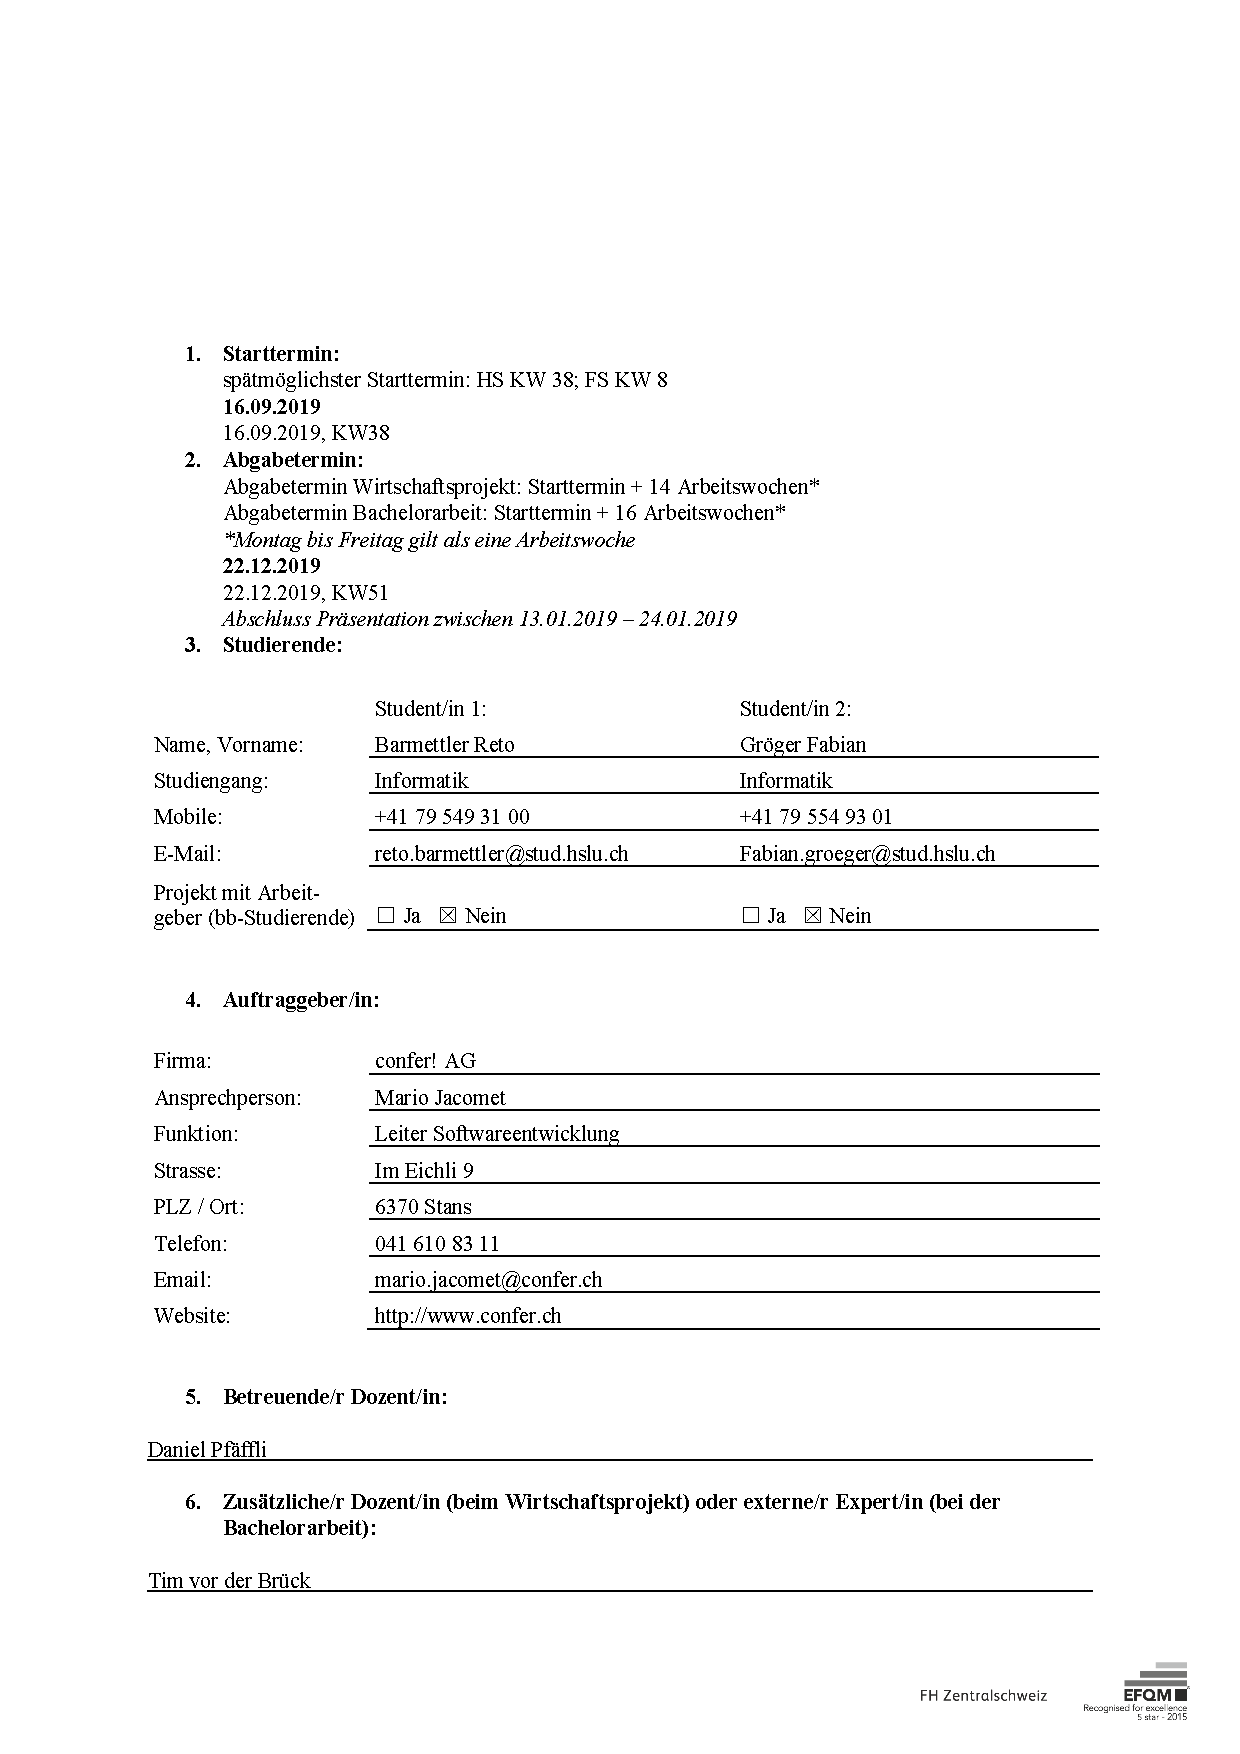
\includepdf[scale=0.75, pages=1, pagecommand=\chapter{Aufgabenstellung Wirtschaftsprojekt}\label{ch:aufgabenstellung}]{img/aufgabenstellung.pdf}
\includepdf[scale=0.75, pages=2-]{img/aufgabenstellung.pdf}


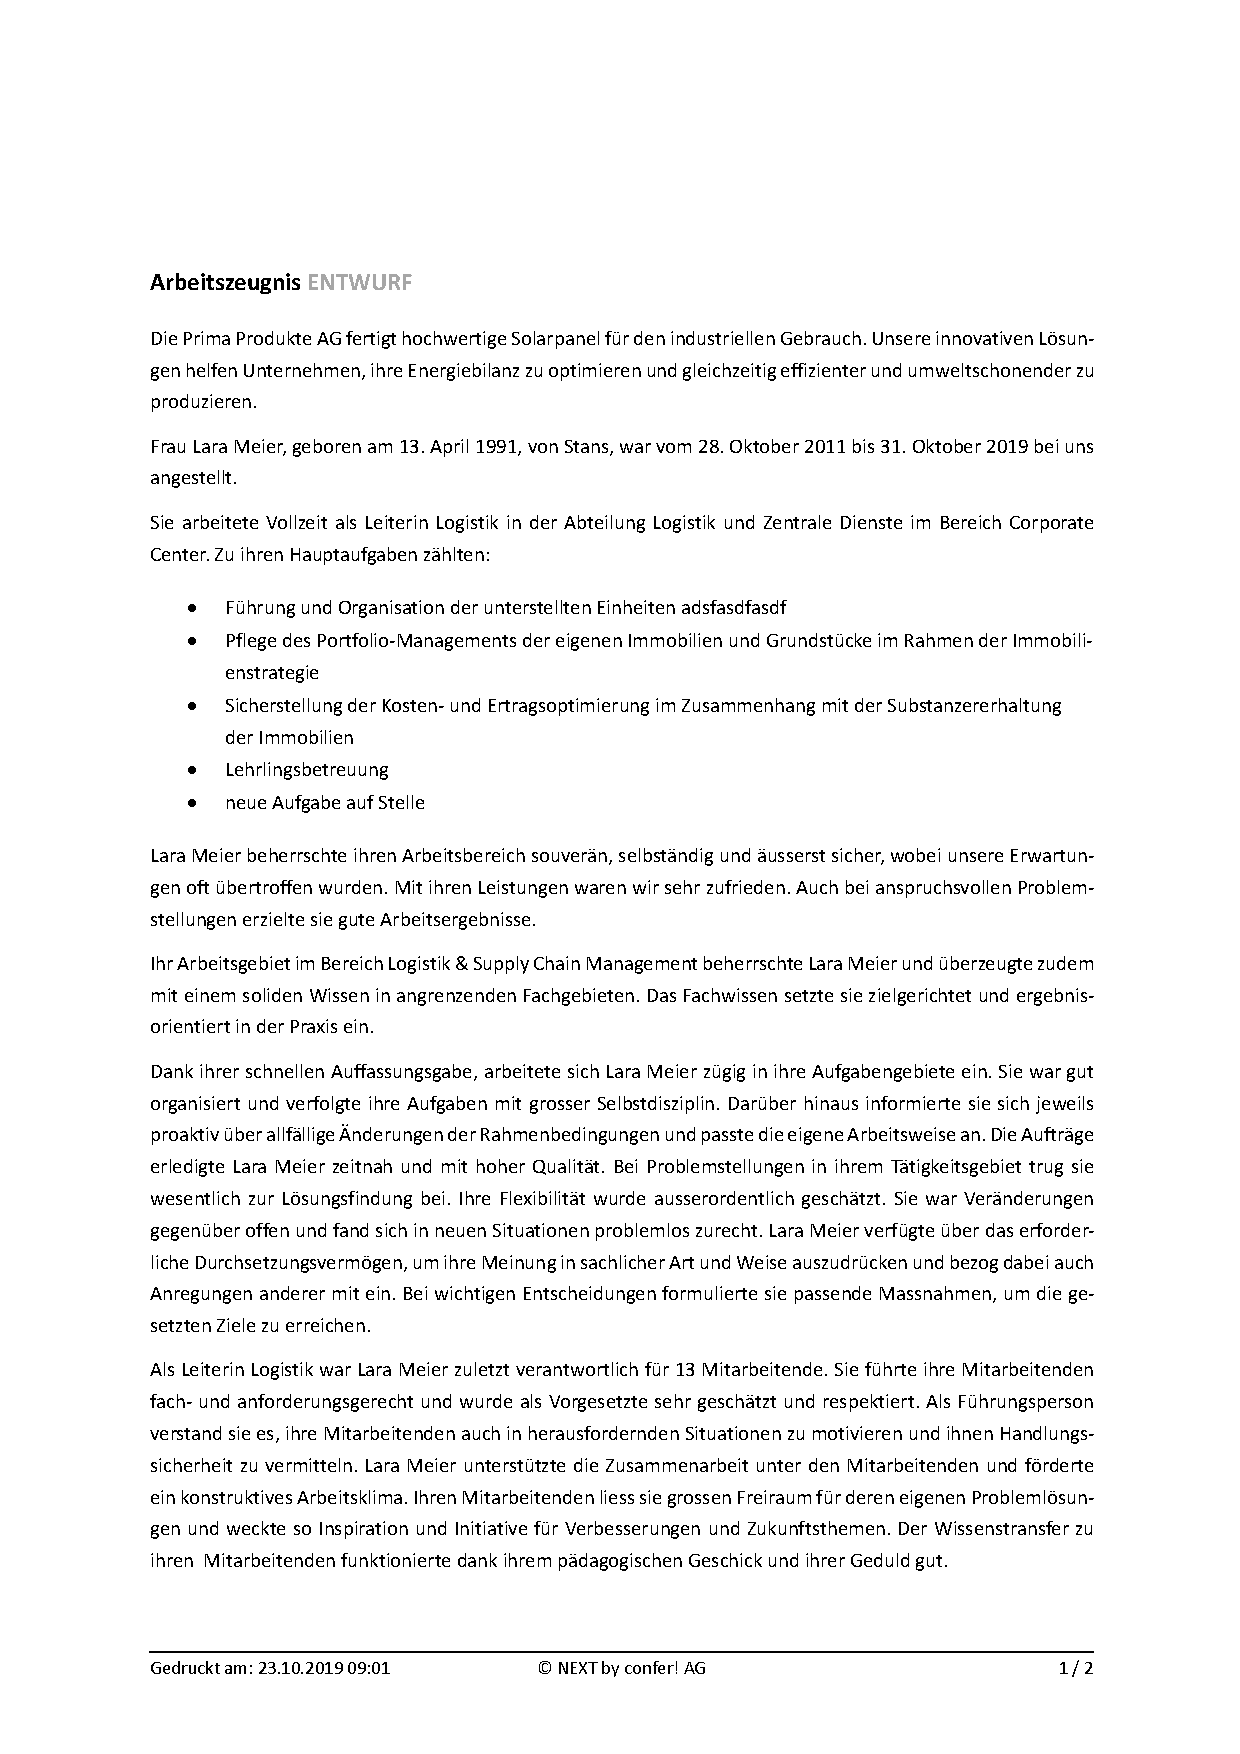
\includepdf[scale=0.75, pages=1, pagecommand=\chapter{Beispiel Arbeitszeugnis Zeugnismanager}\label{ch:beispiel_arbeitszeugnis}]{img/zeugnis_beispiel_zeugnismanager.pdf}
\includepdf[scale=0.75, pages=2-]{img/zeugnis_beispiel_zeugnismanager.pdf}
